\subsubsection{UC13.2 - Visualizzazione del log delle funzioni eseguite}
\begin{figure}[h]
	\centering
	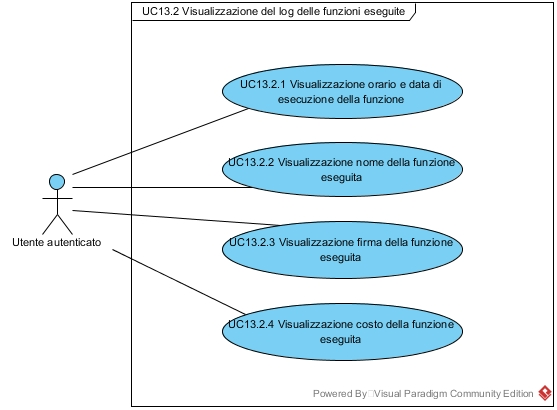
\includegraphics[width=0.7\linewidth]{res/img/UC13.2.jpg}
	\caption{Diagramma UC13.2 - Visualizzazione del log delle funzioni eseguite"}
\end{figure}
\begin{itemize}
	\item \textbf{Attori primari:} Utente autenticato;
	\item \textbf{Descrizione:} l'utente visualizzerà sul \textit{CLI\glo} il risultato del comando "log";
	\item \textbf{Pre-condizioni:} l'utente ha eseguito il comando "log";
	\item \textbf{Post-condizioni:} \textit{CLI\glo} il log relativo alle funzioni da lui eseguite;
	\item \textbf{Scenario principale:} Il sistema mostrerà sulla \textit{CLI\glo} le informazioni relative a tutte le esecuzioni delle funzioni effettuate dall'utente.
\end{itemize}